\documentclass[tikz]{standalone}

\begin{document}
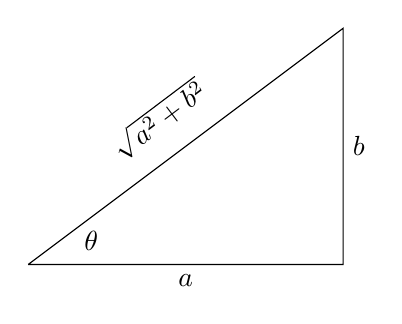
\begin{tikzpicture}
  \draw (0,0) -- (4,0) -- (4,3) -- (0,0);
  \node at (0.8,0.3) {\(\theta\)};
  \node[below] at (2,0) {\(a\)};
  \node[right] at (4,1.5) {\(b\)};
  \node[above, rotate=37] at (1.85,1.6) {\(\sqrt{a^2+b^2}\)};
\end{tikzpicture}
\end{document}
